\section{Results}
The claims this paper defends, each with its interval and its label, are listed in
\texttt{CLAIMS.md}. A claim enters that file only after its report has passed an independent
review by a model from a different vendor with access to the raw records. Sections
\ref{sec:repeat}--\ref{sec:residual} draw only on reports that have passed such a review.
Section~\ref{sec:inreview} reports four studies that are still in that review; every number in it
carries the label \emph{in review}, and none of them is load-bearing for the claims above.
Rates carry the 95\% problem-cluster percentile bootstrap as the primary interval, with the Wilson
interval beside it where the source report gives one, because problems recur across generation
batches and an interval that treats instances as independent is too narrow. The coverage of that
bootstrap under this clustered design with 56 problem clusters has not been validated by
simulation, and every primary interval in this paper inherits that caveat.

Sixteen comparisons were computed in the study that carries the primary contrasts, under one
Bonferroni family with a threshold of $0.00313$. Where a $p$ value appears below, the exact
McNemar value and the cluster-level sign-flip permutation value are both given, because instances
within a problem are not independent and only the second respects that.

\subsection{Returns to repeated reading diminish short of complete}
\label{sec:repeat}

The shipped cross-vendor auditor reads an increment holistically and returns findings; an
increment is blocked if any finding is graded BLOCKER. Over eight independent readings of the same
110 defective instances, union recall rises from 10.7\% at one reading to 30.0\% [20.0, 40.7] at
eight. The eighth reading still adds 1.93 points, cluster [1.14, 2.78], against the flattening bar
of 1.0 points registered before the first model call. The bar was not met. The constrained fit
puts the asymptote at 31.5\%, but on our own registered criterion that figure is an extrapolation
and the raw union at eight readings is the number to quote. What the data support is diminishing
returns at the budget we could afford, not saturation: at 1.9 points per reading the curve was
still climbing when we stopped. That bar is also a function of where a family was stopped, so
families run only to $K = 4$ meet it more easily than families run to $K = 8$, and a curve that
meets it at a small $K_{\max}$ is making a weaker statement than one that meets it at a large one.
Twenty readings pooled across three auditor families reach 48.2\% [36.7, 60.0].

The price is measured on the same footing. Union false positives on 150 correct increments reach
16.0\% [10.1, 22.3] at eight readings, and the recall bought per point of false positive falls
monotonically as readings accumulate.

\begin{figure*}[t]
\centering
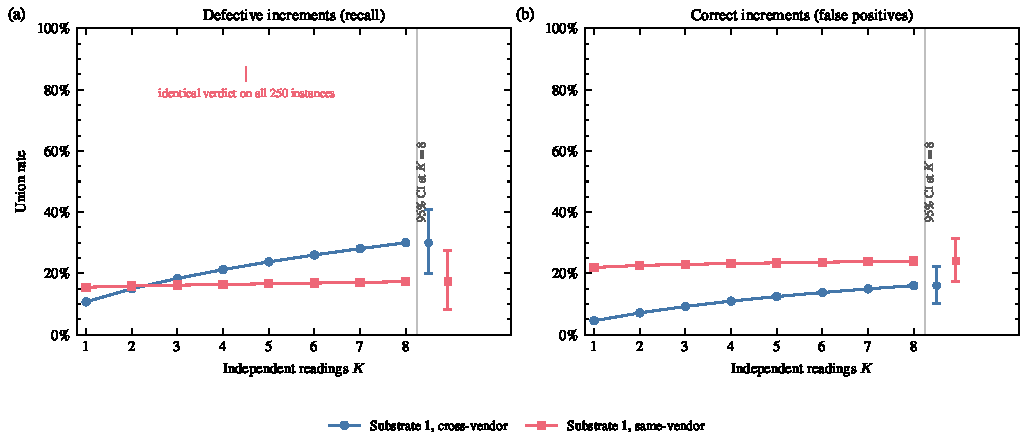
\includegraphics[width=\textwidth]{fig1_saturation.pdf}
\caption{\textbf{Returns to repeated reading diminish short of complete.} Union rate against the
number of independent readings $K$, for two auditor families on substrate 1. (a) recall on
defective increments; (b) false positives on correct increments. Bars at the right of each panel
give the 95\% problem-cluster bootstrap interval of each series at $K=8$, dodged in $x$ so
overlapping intervals stay separable. Neither curve meets the preregistered flattening bar: the
cross-vendor last-step gain is 1.93 points [1.14, 2.78] against a bar of 1.0, so neither is
described as saturating. The same-vendor route is sent temperature $0$ and the cross-vendor route
no sampling parameter at all, so the two unions are not equally free to rise with $K$
(\S\ref{sec:auditor}). A second substrate was plotted here until 2026-09-15 and is withdrawn
(\S\ref{sec:inreview}).}
\label{fig:saturation}
\end{figure*}

\subsection{Which model reads, and under which severity rule}
\label{sec:auditor}

Replacing the auditor with a stronger model of the generator's own vendor moved union recall at
eight readings by $-26.4$ points, cluster $[-37.3, -15.6]$: 4 of 110 against 33 of 110. Three
instances were flagged only by the new family and thirty-two only by the shipped auditor, at an
exact McNemar $p$ of $4.2 \times 10^{-7}$ and a cluster sign-flip $p$ of $2.0 \times 10^{-5}$.
This was a preregistered primary. Three things qualify what it means, all of them measured here
and none of them favourable to reading it as a statement about auditing ability.

First, the two auditors are not at the same operating point, which is the comparison this paper
elsewhere warns against. The stronger model flags correct code at 3.3\% [0.7, 6.7] against the
shipped auditor's 16.0\% [10.1, 22.3]. It blocks less of everything.

Second, the sign reverses under a weaker severity rule. Counting any finding rather than only
findings graded BLOCKER --- an exploratory rule, not preregistered --- the stronger model reaches
59.1\% [47.3, 70.6] on the defect population at 34.0\% [26.5, 41.7] on correct code, against the
shipped auditor's 34.5\% [23.6, 45.5] at 19.3\% [12.8, 26.3]. The ratio of those two rates --- a derived
point ratio we carry no interval for --- is 1.74 and 1.79 respectively, so nothing here shows one
family buying more recall per false positive than the other. The stronger model writes down
more of what is wrong and grades less of it as blocking. The $-26.4$ is a fact about severity
calibration.

Third, the two families are not sampled alike. The shipped cross-vendor route's capability card
does not permit a temperature, so no sampling parameter is sent and the route varies between
readings; the same-vendor route permits one and the layer sends temperature $0$, so that route is
near-deterministic. A union over near-deterministic readings cannot grow, and the two unions are
therefore not equally free to rise. They do not: over $K = 1$ to $8$ the cross-vendor family gains
19.3 points and the same-vendor family gains 3.0. At one reading the gap between them is $-10.1$
points, not $-26.4$; roughly two-thirds of the headline is the difference in how much each union
was permitted to grow. We regard this as the most serious limitation of the contrast, and
\S\ref{sec:limits} records what would be needed to remove it.

A third family argues the other way and belongs beside the headline. A high-reasoning model of the
cross-vendor family reaches 32.7\% [20.7, 45.0] union recall at four readings while flagging
10.7\% [5.9, 16.1] of correct code, dominating the shipped auditor on both axes at half the
readings. So the evidence does not support ``a stronger model is a worse auditor''. It supports
the narrower statement that this particular same-vendor model, at this severity calibration and
sampled at temperature $0$, blocks far less.

A same-vendor auditor of the generator's own size was worse than the cross-vendor one on these
instances by $-12.7$ points $[-25.0, -0.9]$ of union recall at eight readings, signed so that a
negative value favours the cross-vendor auditor. A study on a second substrate reverses that sign,
so this is reported as a measurement on this substrate rather than as a property of same-vendor
auditing.

\subsection{One rulebook sentence moves flags, and does not measurably move outcomes}
\label{sec:rulebook}

Adding a single rule to the auditor's constitution, telling it to find what the visible tests do
not cover, moved flags on the defect population from 10 of 56 to 25 of 56: $+26.8$ points, cluster
[13.6, 40.4], exact McNemar $p = 0.0003$, cluster sign-flip $p = 0.0009$. With the pooled
defect-and-correct flag contrast this is one of only two comparisons that clear the Bonferroni
threshold, and the two are the same effect seen twice.

The estimand is narrower than the sections above and must be read at its own scale. It is measured
on 56 instances from 41 problems, not the 110-instance defect population; it counts flags, not
union recall against the hidden suite; it is one reading, because every loop arm revises once, not
a union over eight; and it is exploratory, because the preregistration named outcome contrasts
rather than flag contrasts. For those reasons we do not compare its magnitude with the $-26.4$ or
the $+19.3$ of the preceding sections, which are union recall at $K=8$ over 110 instances. They
are different quantities on different populations.

Two costs travel with it. On correct code the same rule moved flags by $+12.50$ points [5.17,
21.82], so the sentence makes the auditor louder on both strata. And on the contrast that actually
isolates the rule --- the referent arm against the cross-vendor arm on hidden-suite pass rate after
one revision --- the effect is $+5.36$ points, cluster $[-0.89, +12.07]$, $p = 0.146$, which does
not exclude zero. The rule demonstrably moves what the auditor writes down. Whether that converts
into code that passes the hidden suite is not established, and since this paper argues elsewhere
that a flag is not a catch, that distinction applies to our own intervention first.


\subsection{Most of what the auditor missed is failure the specification never determined}
\label{sec:residual}

Fifty-seven of the 110 defective instances were flagged by no reading of any family. That is a
statement about twenty readings, not about detectability: if an instance is caught with
probability $p$ on each independent reading, twenty readings miss it with probability
$(1-p)^{20}$, which is still $98\%$ at $p = 0.001$ and $36\%$ at $p = 0.05$. Never flagged here
therefore does not mean never flaggable, and we use the residual as a population to characterise
rather than as a set of defects shown to be invisible.

The first classification of that residual asked whether the visible tests exercised the failing
input before it asked anything else. It called 46 of 57 unexercised edges, and an earlier draft of this paper
rested a claim on that.

Re-rating the same instances under a rule that asks first whether the specification's prose
determines the hidden suite's expected value reverses it. Two raters agree that 44 of 57 (77.2\%,
cluster [62.1, 91.1]) are cases where the prose does not settle the value, and that 2 of 57 are
cases where it does and the visible tests merely never built the input. The preregistered
condition for withdrawing ``the residual is mostly unexercised edge'' fires on both of its clauses,
and the claim is withdrawn. The interval is conditional on a category and has no committed
coverage simulation, so it is uncalibrated, as is every category-conditioned interval we report.

A classification that reverses when the order of its questions changes is, by itself, weak evidence
about the auditor, and the raters are not independent of it: one was the author, who wrote the
rubric and knew the earlier labels and which claim was at stake. Three things support the second
reading. The rubric was fixed before any label was written. The labels were committed before we
looked for outside evidence. And when a first pass was found to have carried instance identifiers
and a sheet name into the raters' view, the labelling was re-run with identities stripped and the
result held. Where an outside party had independently recorded that one of these specifications is
defective, in twelve MBPP tasks named in a paper written for another purpose, our raters agree on
9 of the 11 that fall inside our defect population, with both disagreements on the boundary that
paper's own ``incomplete'' category draws. That check is one-sided by construction: it can support
agreement where an outsider looked, and can bound nothing about the rate.

\subsection{Four studies in review, and what their reviews found}
\label{sec:inreview}

Four further studies had reported when this paper was written, and all four were refused quotation
by their independent reviews on the same day. We report that outcome rather than their numbers,
because two of the refusals bear on how far the results above reach.

\textbf{A second substrate, withdrawn.} This paper reported a second benchmark until its review
refused quotation, and we then confirmed the reason ourselves: the visible-test text shown to the
auditor \emph{and} to the generator was sliced out of its test class without the class header, so
it failed to parse on all 300 tasks, while scoring executed the intact class. Both models read
invalid Python on every task of that substrate. An auditor shown a broken test file can return a
finding about the file rather than about the candidate, which raises the flag rate on both strata at
once and so inflates recall and false positives together; the finding texts were not archived, so no
reading can be reclassified after the fact. The extraction is fixed and the study is registered for
a re-run whose numbers we will report whichever way they move.

\textbf{A prospective test of the residual, withdrawn.} We constructed a population of injected
defects intended to make specification-determinedness hold by construction. Review established that
it does not: the filter we registered to recover each edit's first failing hidden input was
implemented as a check that the injector had written a non-empty string, and no check connects the
quoted specification text, the named input class, the witness and the actual failure. What the
population contains is small edits that survive a sparse visible suite and fail a hidden one, and a
preregistered probe separates them from natural code at 96.7\%. The auditor does block them far
more often than it blocks the natural residual, but the two populations differ in more than the
property we meant to isolate, so this is not the prospective test of \S\ref{sec:residual} and we
do not offer it as one.

\textbf{Two others.} A study of what a flag is worth, and a study of whether a changed rulebook
moves a second vendor's family, were both refused for overstating what their measurements
establish; their corrections do not change any number quoted above.

We report these outcomes because a paper that makes evidentiary discipline its method should show
the gate rejecting its own work, not only passing it. None of the numbers in
\S\ref{sec:repeat}--\S\ref{sec:residual} depends on any of these four studies.

\subsection{What follows for a recall number}

Taken together, the results above say an audit recall figure is a joint property of the auditor
and its material. It moves with which model reads, with what the rulebook tells it to look for,
and with whether the benchmark's hidden suite asks a question the specification answers. It also
moves with the severity threshold at which a finding becomes a block, and with how the route is
sampled, neither of which is usually reported.
